\section{Evaluation}
To evaluate the impact flat combining has on the global data structures, we ran a series of experiments to test the raw performance of the data structures themselves under different workloads, and further measured their impact on performance of two simple graph benchmarks.

\subsection{Data Structure Throughput}
First we measured the performance of the global data structures on extremely simple workloads to understand their raw performance.

\begin{figure*}[t]
  \centering
  \begin{subfigure}[b]{0.9\textwidth}
  \centering
  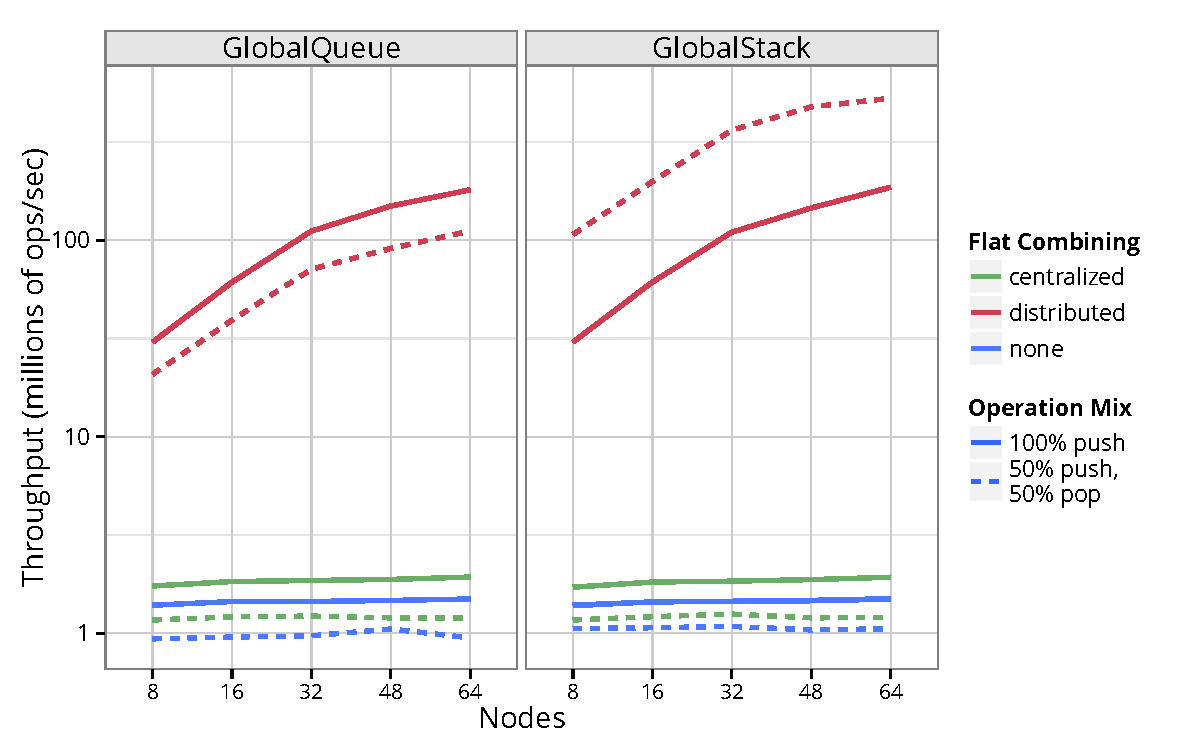
\includegraphics[width=\textwidth]{data/plots/vector_perf.pdf}
  \caption{\emph{GlobalStack and GlobalQueue.}
    Results are shown on a log scale for a throughput workload performing 256 million operations with 2048 workers per core and 16 cores per node. Flat combining improves throughput by at least an order of magnitude and allows performance to scale. Matching pushes and pops enables the stack to perform even better on a mixed workload.
  }
  \label{fig:vector}
  \end{subfigure}%
  % \hspace{0.05\textwidth}
  % % ~ %add desired spacing between images, e. g. ~, \quad, \qquad etc.
  % %(or a blank line to force the subfigure onto a new line)
  % \begin{subfigure}[b]{0.45\textwidth}
  % \centering
  % 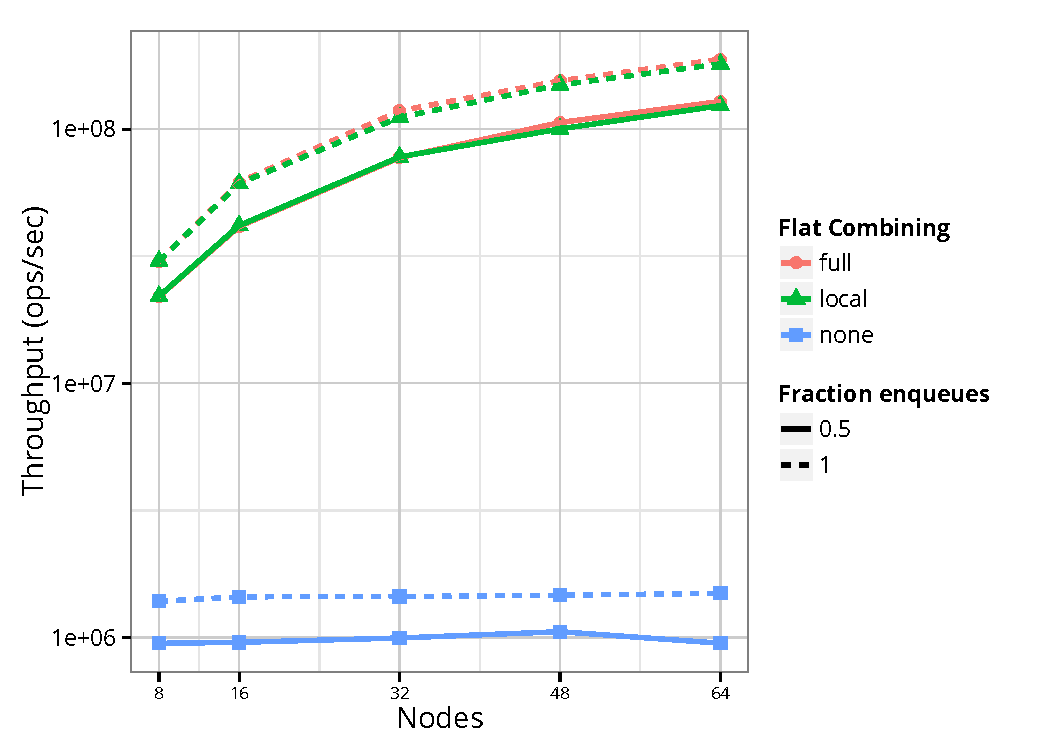
\includegraphics[width=\textwidth]{data/plots/queue_perf.pdf}
  % \caption{\emph{GlobalQueue.} Same parameters as stack performance results. The queue is unable to do matching locally, but benefits from reducing the amount of synchronization that must globally serialize. The mixed workload performs worse because the current implementation serializes combined enqueue and dequeue operations.}
  % \label{fig:queue}
  % \end{subfigure}
  % \hspace{0.05\textwidth}
  
  %  
  \begin{subfigure}[b]{0.9\textwidth}
  \centering
  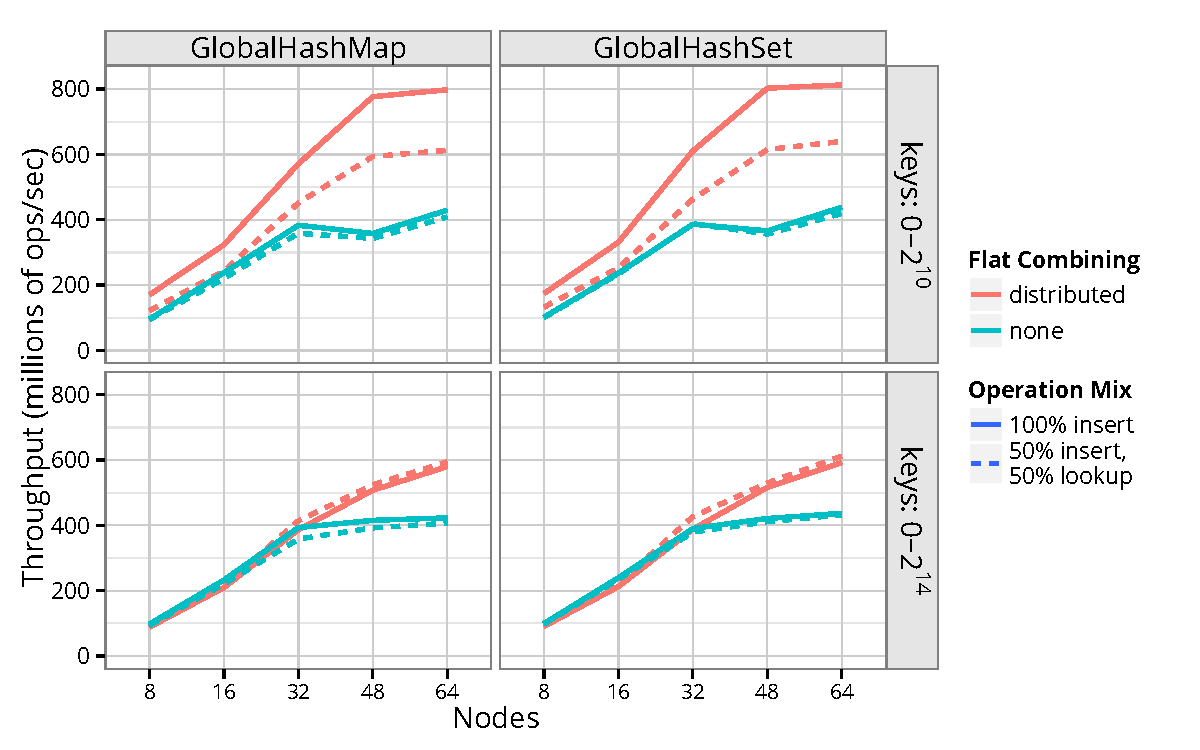
\includegraphics[width=\textwidth]{data/plots/hash_perf.pdf}
  \caption{\emph{GlobalHashSet and GlobalHashMap.}
    Results are shown for a throughput workload inserting and looking up 256 million random keys in the range 0-1024 into a global hash with 1024 cells. 
    Performance without combining scales out to 32 nodes because synchronization happens at each hash cell, but drops off as the number of destinations increases. Due to eliminating duplicate inserts and lookups, the combining version is able to continue to scale.}
    \TODO{if time: add 'delete' operation, too (show that it doesn't affect correctness or performance)}
  \label{fig:hash_perf}
  \end{subfigure}
  % %
  % \hspace{0.05\textwidth}
  % %
  % \begin{subfigure}[b]{0.45\textwidth}
  % \centering
  % 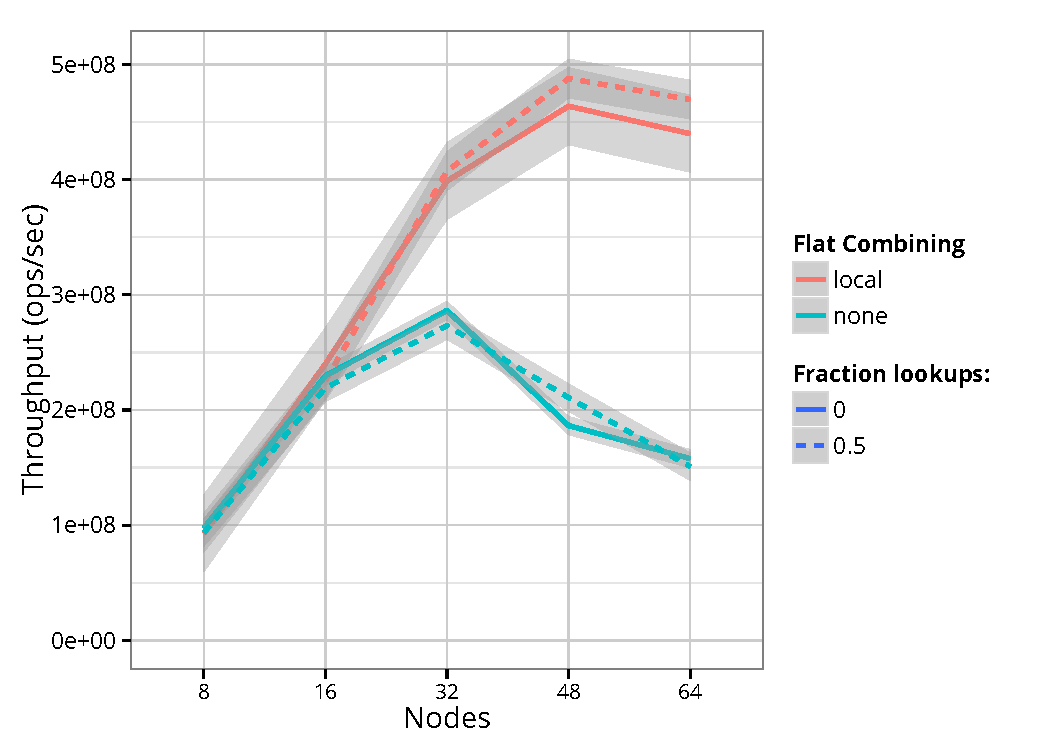
\includegraphics[width=\textwidth]{data/plots/hashmap_perf.pdf}
  % \caption{\emph{GlobalHashMap.} Same workload as for the Set, but random integers as the values in the map. Performance matches that of the Set.} \TODO{try increasing size of value "payload", currently is just a tiny int64.}
  % \label{fig:hashmap}
  % \end{subfigure}%
  %
  \caption{
    \emph{Raw performance of global data structures on simple throughput workloads.}
    Results shown for workloads with varying mixtures of writing and reading operations. All experiments were performed with 16 cores per node, and a suitable set of Grappa runtime parameters fixed for a given plot.
    \TODO{either all with error bars or none?}
    \TODO{combine stack/queue \& set/map plots, no point in saying the same things twice.}
  }\label{fig:datastructs}
\end{figure*}

\paragraph{Queue and Stack}
The GlobalQueue and GlobalStack have very similar implementations in terms of how they are synchronized. Even with Grappa's aggregation, without combining, both the stack and queue completely fail to scale because of serialization of all workers' updates on the master core.
With combining, both scale well out to 64 nodes.
On the mixed workload, the stack is able to do matching locally, allowing it to reduce the amount of communication drastically, greatly improving its performance.

The queue also benefits from reduced synchronization and batching operations, and its all-push workload performs identically to the stack's.
However, the queue is unable to do matching locally, and in fact, the mixed workload performs worse because the current implementation serializes combined enqueue and dequeue operations. This restriction could be lifted with more careful synchronization at the master core allowing enqueues and dequeues to proceed in parallel as long as they do not conflict.

\paragraph{HashSet and HashMap}
The GlobalHashSet and GlobalHashMap have the same synchronization strategy (serialization happens at each hashed location).
Performance without combining scales better than the global queue or stack because synchronization happens at each hash cell, but drops off as number of destinations increases. Combining version is able to match inserts and lookups of the same key, enabling it to have a steeper scaling curve.

\subsection{Application Kernel Performance}
The impetus for this work was that naive implementations of standard data structures are insufficient for use in high-performance kernels.

\paragraph{Breadth-First Search}
\begin{figure}[t]
  \centering
  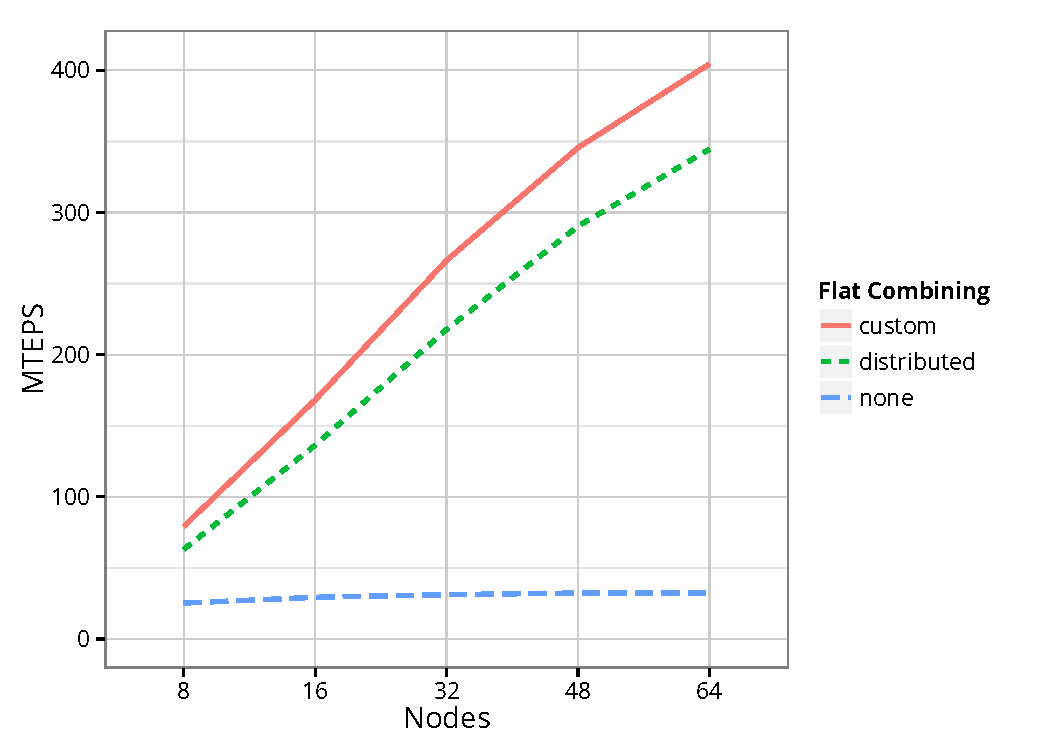
\includegraphics[width=0.5\textwidth]{data/plots/bfs_perf.pdf}
  \caption{\emph{BFS} on a Graph500-spec graph of scale 26 (64 million vertices, 1 billion edges), with the direction-optimizing BFS algorithm. Performance is measured in millions of Traversed Edges Per Second (MTEPS).}
  \label{fig:bfs_perf}
\end{figure}


\paragraph{Connected Components}

\begin{figure}[t]
  \centering
  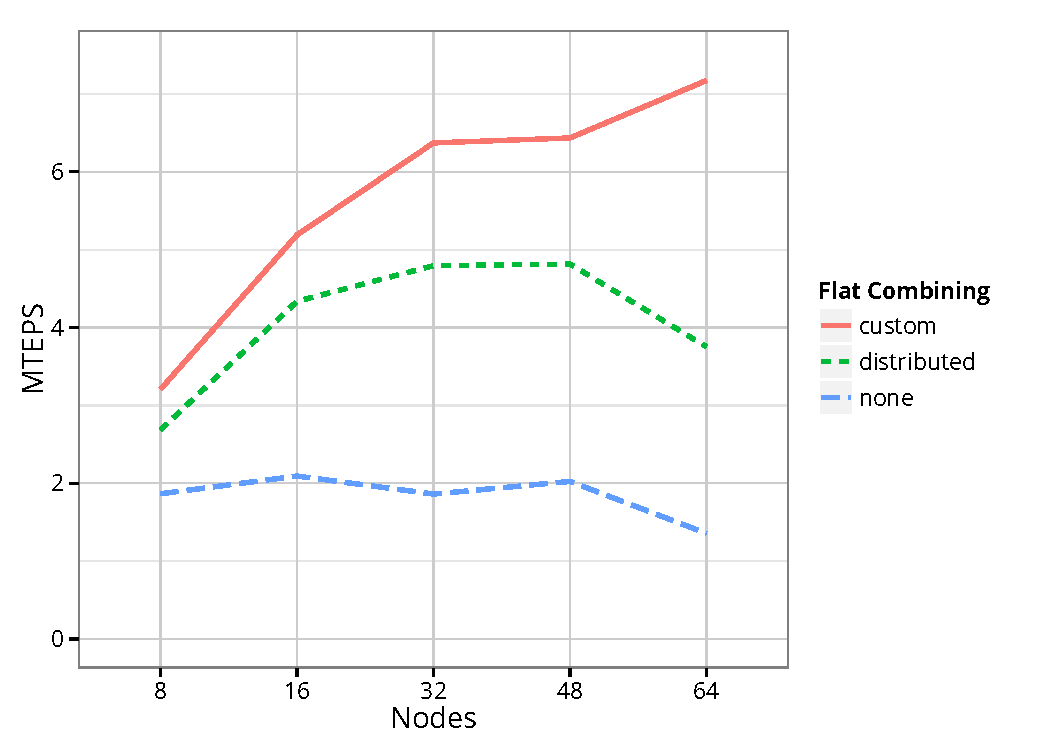
\includegraphics[width=0.5\textwidth]{data/plots/cc_perf.pdf}
  \caption{\emph{Connected Components} on the same scale 26 Graph500 graph. Performance is measured in MTEPS (parameterized by the total number of edges in the graph, independent of the algorithm used).}
  \label{fig:cc_perf}
\end{figure}

